\subsection*{Диаграмма развертывания приложения}

UML диаграмма развертывания (deployment diagram) - это один из типов диаграмм UML, который используется для моделирования аппаратного обеспечения и программных компонентов системы,
а также для их взаимодействия и развертывания на различных устройствах.

Диаграмма развертывания показывает физическую структуру системы, включая сервера, устройства хранения данных, сети и другое оборудование.
Компоненты системы, а также их зависимости и связи, также отображаются на диаграмме.

Диаграмма развертывания может быть полезна для проектирования системы, позволяя определить необходимое оборудование, на котором будет развернута система,
а также понять, как различные компоненты системы будут взаимодействовать друг с другом и с окружающей средой.

Диаграмма развертывания приложения спроектирована в draw.io \cite{drawio} и представлена на рис.~\ref{fig:UML_deployment_diagram}.

\begin{figure}[!htb]
    \centering

    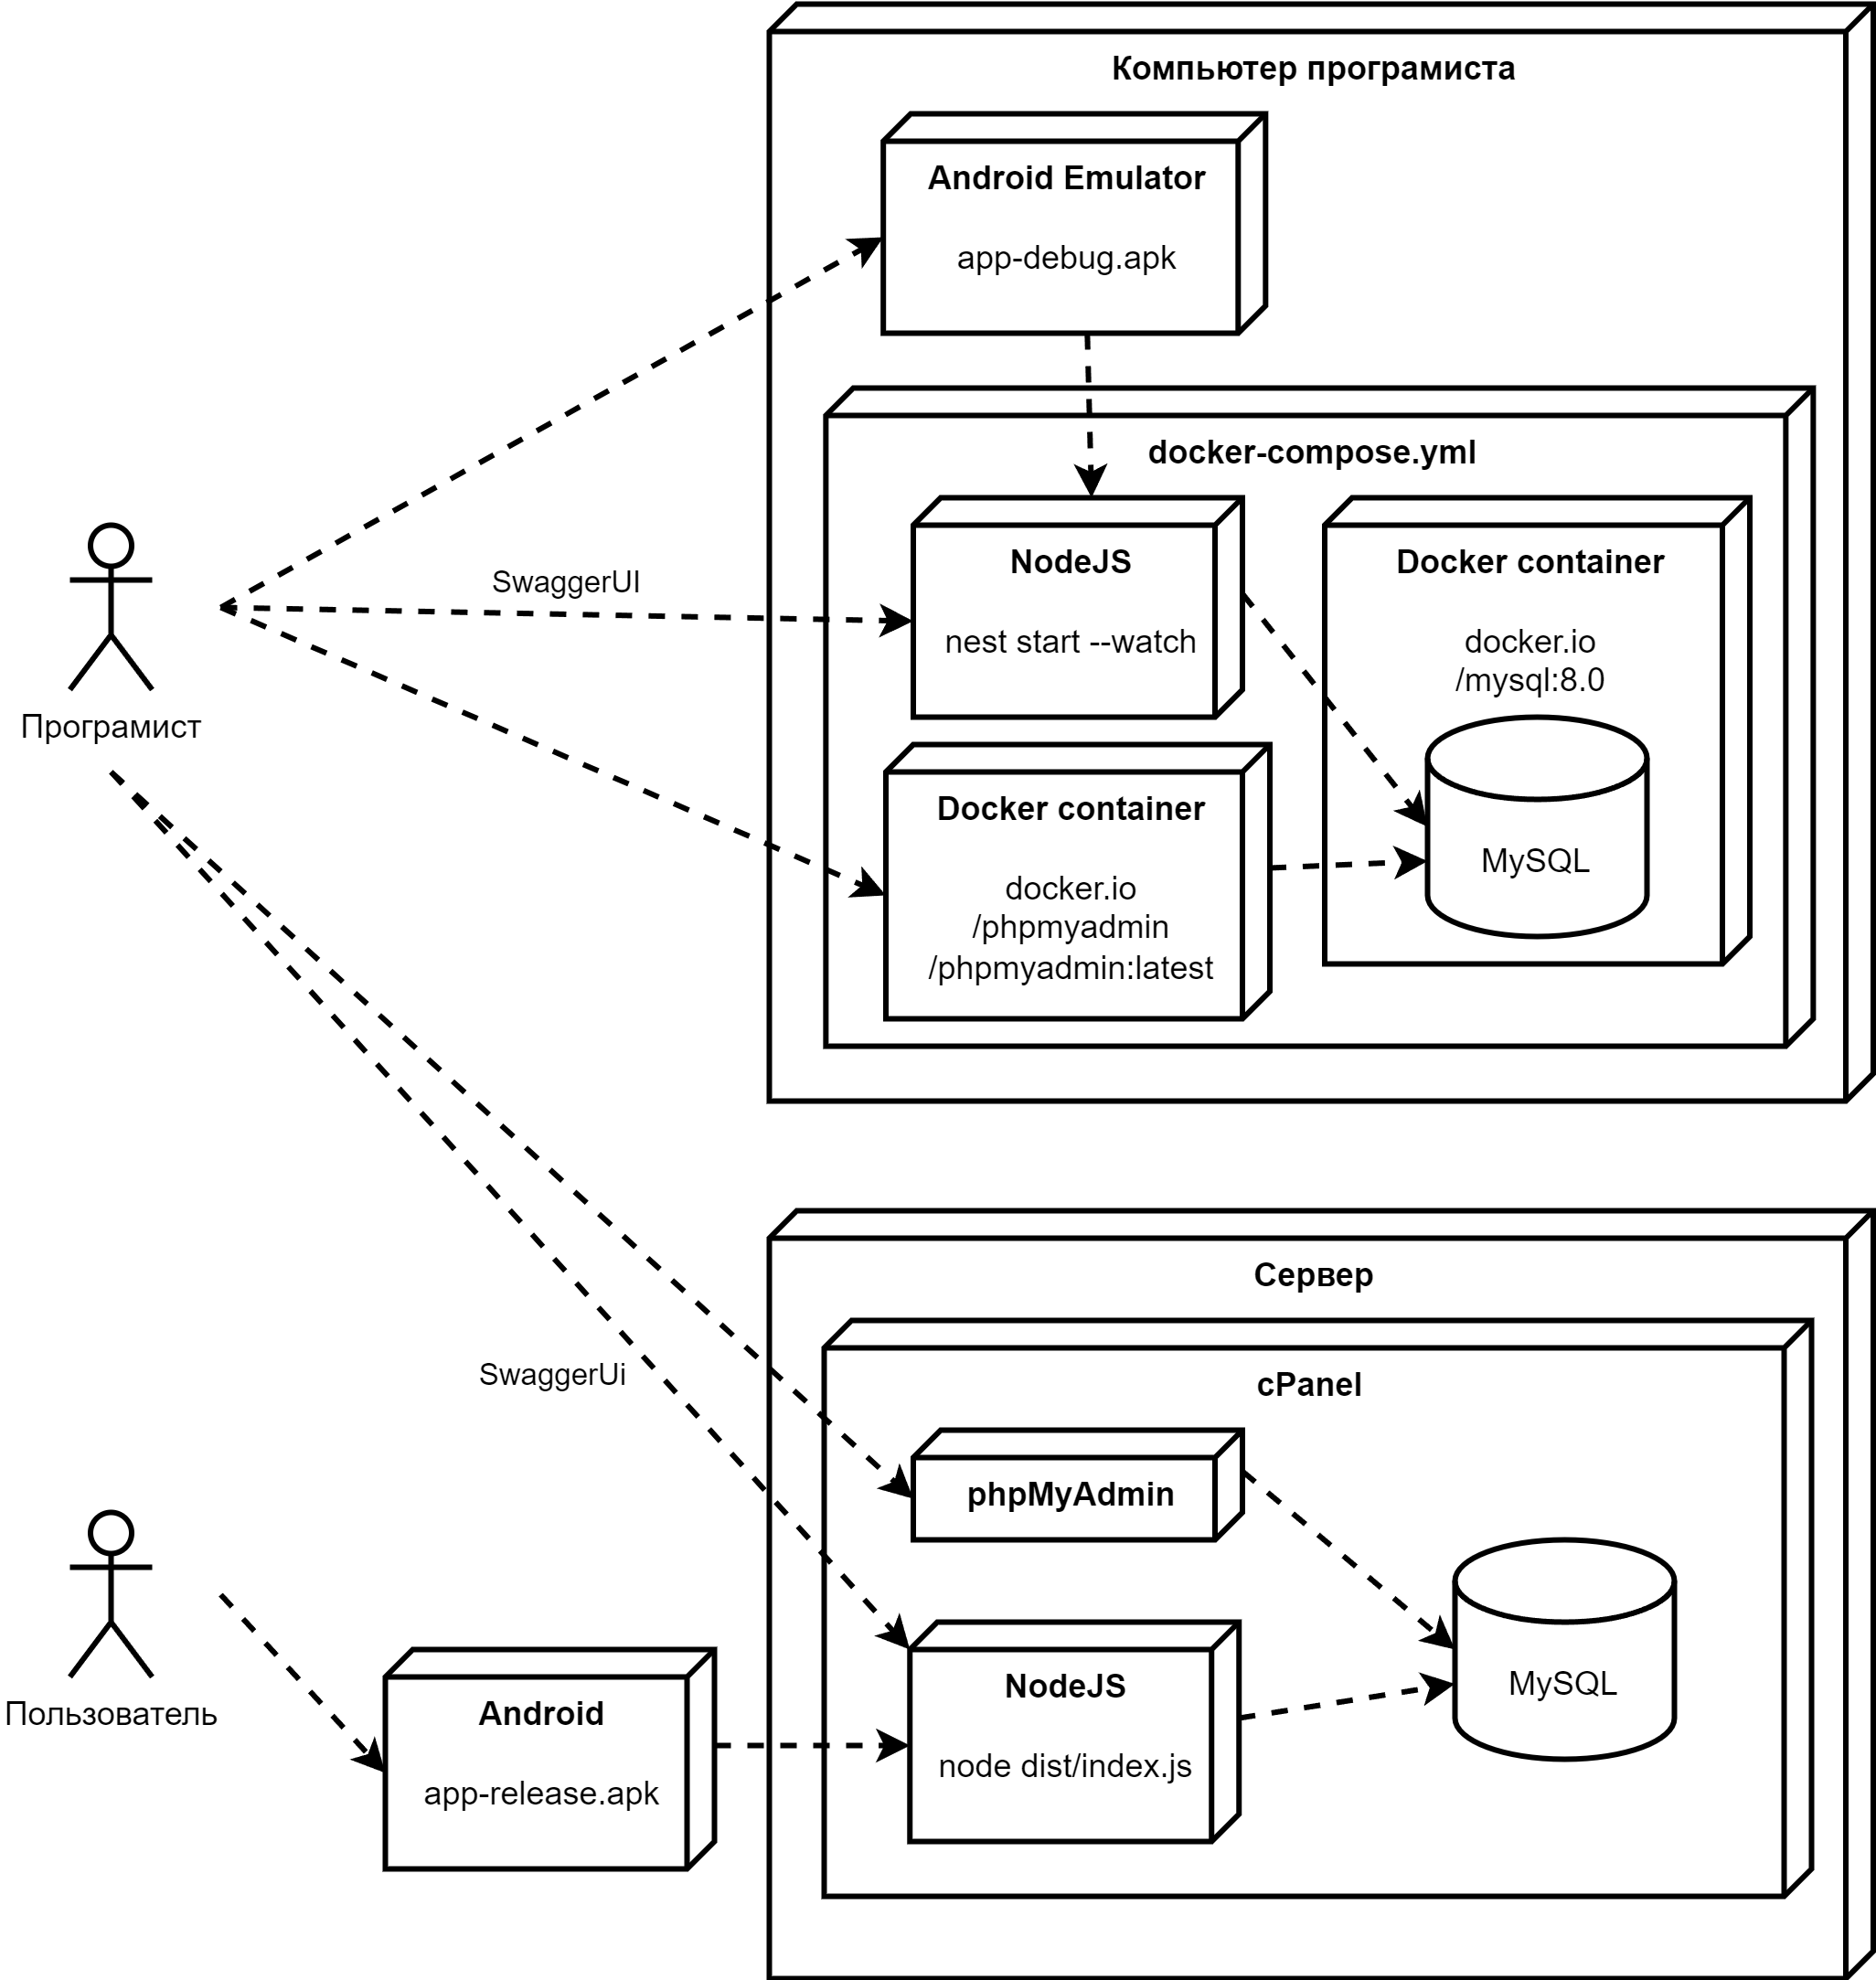
\includegraphics[width=18cm]
    {images/UML/UML_deployment_diagram.png}

    \caption{Диаграмма развертывания приложения}

    \label{fig:UML_deployment_diagram}
\end{figure}
